\documentclass[12pt]{report}

\usepackage{times}
\usepackage{xcolor}
\usepackage{dirtree}
\usepackage{graphicx}
\usepackage{hyperref}
\usepackage{indentfirst}
\usepackage[margin=1in]{geometry}

\hypersetup{colorlinks=true, linkcolor=teal}
\setlength{\DTbaselineskip}{25pt}
\renewcommand{\DTstyle}{\rmfamily\large}

\newcommand{\n}{\par}
\newcommand{\br}{\vspace{1 em}\n}

\title{SBA Web Application Report}
\author{David W.}
\date{Last Revised \today}

\begin{document}
\maketitle

\textbf{Introduction}
\br
This report discusses Assignee, a web application developed to fulfill the SBA task of implementing an assignment system.
\br
This report includes the following chapters on various aspects:
\begin{itemize}
	\item \hyperref[overview]{Overview}:\\
	      Project objectives and structure;
	\item \hyperref[data-layer]{Data Layer}:\\
	      Relational database design and implementation;
	\item \hyperref[application-layer]{Application Layer}:\\
	      Design and implementation of site back-end components;
	\item \hyperref[presentation-layer]{Presentation Layer}:\\
	      Design and implementation of site front-end components;
	\item \hyperref[security]{Security}:\\
	      User authentication and cross-layer interaction security;
	\item \hyperref[accessibility]{Accessibility}:\\
	      Considerations for site accessibility and localization (l10n);
	\item \hyperref[performance]{Performance}:\\
	      Optimizations for application performance;
	\item \hyperref[quality-assurance]{Quality Assurance}:\\
	      Unit and integration testing;
	\item \hyperref[tools-used]{Tools Used}:\\
	      Applications, extensions, packages, and libraries utilized during development;
\end{itemize}
\tableofcontents

\chapter{Overview} \label{overview}
\section{Project Objectives} \label{overview.project-objectives}
The following pages provide a brief overview of user capabilities by role.
We have three core systems - User, Team, and Assignment - designed to manage complex application logic, as detailed below.
\br
Notes:\n
Only workflow-related points are included; GUI aspects are excluded.\n
Each task is described broadly (e.g., login), with detailed information provided later in the report.
\br
Symbolic Notes:\n
...... $\rightarrow$ \{A\}: The user performing the action attains role A.\n
\{B\} $\rightarrow$ \{C\}: The action allows a user with role B to attain role C.\n
\{D\} $\in$ \{E\}: Role D inherits from role E, granting users with role D all permissions of role E.
\subsection{User System} \label{overview.project-objectives.user-system}
Roles: \{Site Visitors\}, \{Logged-in Users\}\n
\begin{itemize}
	\item \{Site Visitors\}
	      \begin{itemize}
		      \item Register for accounts;\null\hfill $\rightarrow$ \{Logged-in Users\}
		      \item Log in to existing accounts;\null\hfill $\rightarrow$ \{Logged-in Users\}
	      \end{itemize}
	\item \{Logged-in Users\}
	      \begin{itemize}
		      \item Change password;
		      \item Change username or email;
		      \item Modify other settings;
		      \item Log out;\null\hfill $\rightarrow$ \{Site Visitors\}
		      \item Delete account;\null\hfill $\rightarrow$ \{Site Visitors\}
	      \end{itemize}
\end{itemize}\n
The User System is a standard account management system found in web applications.
It allows visitors to create accounts, while registered users can log in and manage their account settings.
\br
Authentication techniques are implemented to support this system, with detailed information provided in later chapters.
\br
The User System is central to all components of this application,
including the Team System, the Assignment System, and any future systems that may be introduced,
such as a Posts and Comments System or an Instant Messaging System using P2P WebRTC or C/S WebSockets.
\subsection{Team System} \label{overview.project-objectives.team-system}
Roles: \{Users\}, \{Team Members\}, \{Team Monitors\}, \{Team Owners\}\n
\begin{itemize}
	\item \{Users\}
	      \begin{itemize}
		      \item Join teams;\null\hfill $\rightarrow$ \{Team Members\}
		      \item Create teams;\null\hfill $\rightarrow$ \{Team Owners\}
	      \end{itemize}
	\item \{Team Members\} $\in$ \{Users\}
	      \begin{itemize}
		      \item Leave the team;\null\hfill $\rightarrow$ \{Users\}
		      \item Comment on messages*;
	      \end{itemize}
	\item \{Team Monitors\} $\in$ \{Team Members\}
	      \begin{itemize}
		      \item Invite team members;\null\hfill \{Users\} $\rightarrow$ \{Team Members\}
		      \item Kick team members;\null\hfill \{Team Members\} $\rightarrow$ \{Users\}
		      \item Post messages*;
	      \end{itemize}
	\item \{Team Owners\} $\in$ \{Team Monitors\}
	      \begin{itemize}
		      \item Change team name;
		      \item Change team description;
		      \item Appoint team monitors;\null\hfill \{Users\} $\rightarrow$ \{Team Monitors\}
		      \item Remove team monitors;\null\hfill \{Team Monitors\} $\rightarrow$ \{Users\}
		      \item Delete the team;\null\hfill $\rightarrow$ \{Users\}
	      \end{itemize}
\end{itemize}\n
Similar to Google Classroom, users can create or join teams,
with team owners having the ability to appoint or remove team monitors to assist in managing the team.
Additionally, roles within the hierarchy can manage members and perform team actions to varying degrees and extents.
\br
The *post and comment features are not implemented in the initial version of the web app, as they are considered a lower priority.
If these features are added later, they will be decoupled from the current system.
\br
The Team System is central to the \hyperref[overview.project-objectives.assignment-system]{Assignment System}.
\subsection{Assignment System} \label{overview.project-objectives.assignment-system}
Roles: \{Team Owners\}, (\{Team Members\},) \{Assignees\}\n
\begin{itemize}
	\item \{Team Owners\}
	      \begin{itemize}
		      \item Author assignments;
		      \item Add attachments to assignments;
		      \item Assign assignments;\null\hfill \{Team Members\} $\rightarrow$ \{Assignees\}
		      \item Revoke assignments;\null\hfill \{Assignees\} $\rightarrow$ \{Team Members\}
		      \item Grade, comment on, and return submissions;
	      \end{itemize}
	\item \{Assignees\} $\in$ \{Team Members\}
	      \begin{itemize}
		      \item Submit assignments;
		      \item Add attachments to submissions;
	      \end{itemize}
\end{itemize}\n
The Assignment System is the core feature we are tasked with completing. The system operates intuitively:\n
Team owners can assign assignments to selected team members with a deadline.
Assignees can draft and submit their work.
After submission, the team owner can grade the assignment, provide comments, and return it to the assignee.
\br
An attachment system is designed to manage attachment files,
enabling team owners and assignees to add additional files to their assignments and submissions without needing to reattach all previous files after exiting.
More details will be provided in later chapters.
\section{Project Structure} \label{overview.project-structure}
\subsection{Folder Structure} \label{overview.project-structure.folder-structure}
To maintain a clear separation of concerns and promote modularity, the web application is divided into three layers,\n
Data Layer: Manages data storage and retrieval;\n
Application Layer: Contains the business logic and processes data;\n
Presentation Layer: Handles user interface and user interaction;
\br
This organization can be observed in the project folder structure.
While the folder structure may undergo frequent changes, its fundamental layout will remain consistent across revisions.
\newpage
\dirtree{%
	.1 /.
	.2 design/.
	.3 database/.
	.3 report/.
	.2 site/.
	.3 backend/.
	.3 frontend/.
}
\vspace{2 em}
The design/ directory contains files that are not part of the actual web application.
This includes the report, media assets used in the report, and other related documents.
\br
Notes:\n
The database/ directory corresponds to the Data Layer.
It is located under design/ because the hosted database is independent of the site/ folder (linked only via the database URL in the .env file).
Only the distribution .sql file used to instantiate the database is stored here.
Further details can be found in the chapter \hyperref[data-layer]{Data Layer}.
\br
The directory backend/ corresponds to the Application Layer.
Further details can be found in the chapter \hyperref[application-layer]{Application Layer}.
\br
The directory frontend/ corresponds to the Presentation Layer.
More information is provided in the chapter \hyperref[presentation-layer]{Presentation Layer}.
\subsection{Repository} \label{overview.project-structure.repository}
The entire project folder is hosted in a repository available at
\href{https://github.com/CarbonicSoda/assignee}{GitHub/Carbonic\-Soda/assignee} for inspection.
\br
With GitHub, we can review all past commits from the start of this project to the latest update or patch.
This functionality not only facilitates version control and debugging but also enables simultaneous work on the back-end and front-end through branching.

\chapter{Data Layer} \label{data-layer}
This chapter covers the design and implementation of the supporting relational database.
\br
In the section \hyperref[data-layer.design]{Design}, we discuss the design of tables, fields, and their data types, along with the rationales behind these choices. We also explore the relational mappings of tables and fields from multiple perspectives. Finally, we will delve into the adoption of normal forms in greater detail.
\br
%MO DEV unfinished
% In the section \hyperref[data-layer.implementation]{Implementation}
\section{Design} \label{data-layer.design}
The design of the relational database follows the blueprint outlined in the section \hyperref[overview.project-objectives]{Project Objectives}.
The three core systems and their related entities (roles) are utilized to structure and populate the database.
\br
Notes:\n
Throughout the database, lowercase is used for table and field names, in contrast to conventional practices.
This choice helps distinguish entities from SQL commands, which are typically written in uppercase.\n
When not otherwise specified (Null-able), all table attributes are defined as Not Null.
This approach is taken to prevent potential issues related to database consistency that can arise from having Null entries.
It reduces the risk of anomalies in data retrieval, and simplifies backend application logic dealing with complicated queries.
\subsection{User System} \label{data-layer.design.user-system}
The User System serves as the backbone of the entire web application, responsible for storing user account-related data.
This system encompasses user identifiers, user preferences, and authentication data.
\br
In Assignee, users can register for accounts using their email addresses.
The email address acts as the unique identifier for user login.
This approach simplifies the process, eliminating the need for users to create a username,
as their email is readily available for use.
\br
While logging in with their email addresses, users can choose their own display names for better identification.
These display names do not need to be unique, allowing users the flexibility to select names that resonate with them.
\br
\begin{figure}
	\centering
	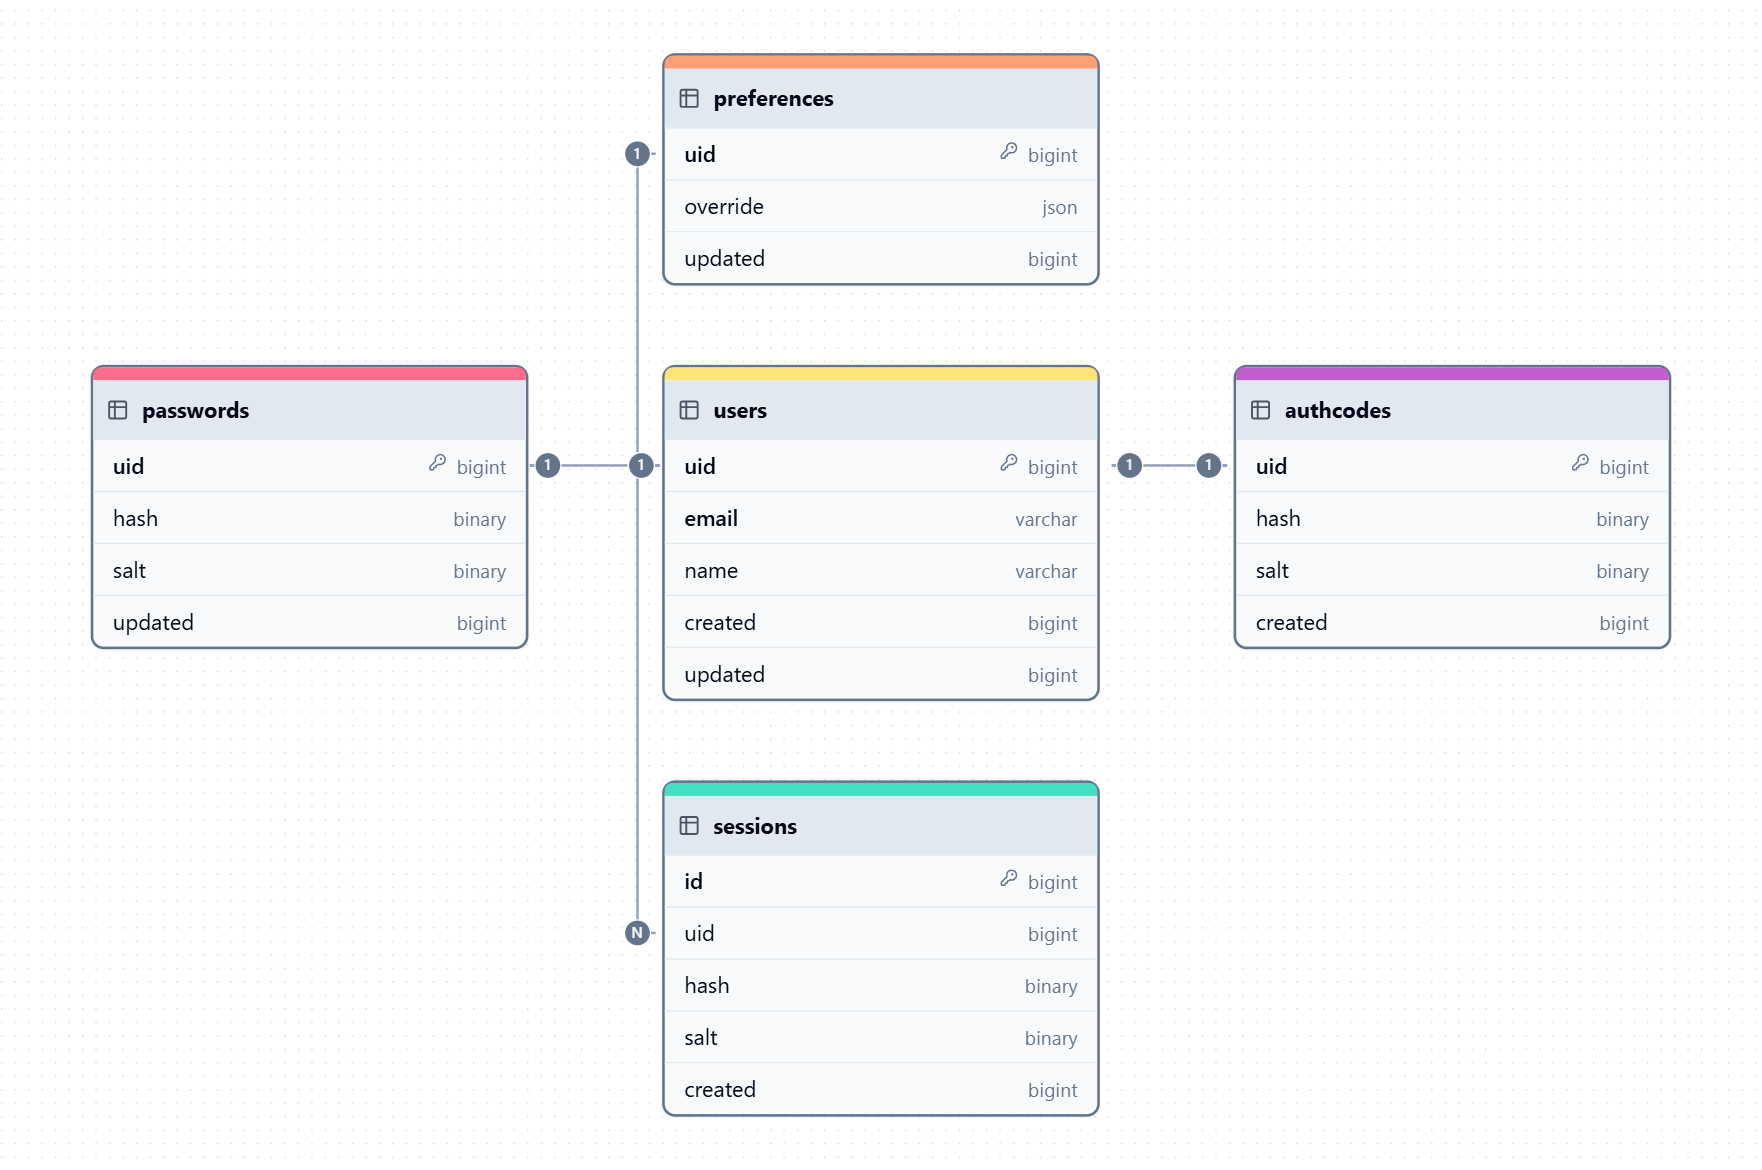
\includegraphics[width=\linewidth]{user_system.jpeg}
	\caption{User System ER Diagram}
	\label{fig:user-system-er}
\end{figure}
The User System consists of five tables, as described below,
\begin{itemize}
	\item users: Contains user account identification information;
	\item preferences: Stores user preferences;
	\item authcodes: Holds user email authentication codes;
	\item passwords: Manages user password information;
	\item sessions: Tracks user browser sessions;
\end{itemize}
\subsubsection{Table - users} \label{data-layer.design.user-system.users}
- uid (Primary Key) (BIGINT UNSIGNED) (Auto-Increment)\n
Although the email address is a candidate key for the table, uid is chosen as the primary key for several reasons:\n
\begin{itemize}
	\item Storage Efficiency: Tables referencing a user can save on storage space by using a BIGINT instead of a VARCHAR.
	\item Indexing Performance: Indexing this frequently accessed table is typically faster with a BIGINT.
	\item Consistency and Flexibility: Using an auto-increment primary key helps maintain database consistency and flexibility, especially if there comes a time when email login is no longer used.
\end{itemize}\n
The BIGINT is set to be unsigned to maintain consistency across the application.
This approach prevents potential issues in backend logic that could arise from wrapped negative numbers,
ensuring stability and reliability in data handling.
\br
- email (Unique) (VARCHAR(254) ASCII)\n
The unique email address used for account registration and login is defined as VARCHAR type in the database schema. This choice accommodates the flexible length of email addresses.\n
VARCHAR is capped to 254 characters in ASCII, this is to align with the standards outlined in
\href{https://www.rfc-editor.org/rfc/rfc5322}{RFC 5322: Internet Message Format}.
\br

% \chapter{Application Layer} \label{application-layer}

% \chapter{Presentation Layer} \label{presentation-layer}

% \chapter{Security} \label{security}

% \chapter{Accessibility} \label{accessibility}

% \chapter{Performance} \label{performance}

% \chapter{Quality Assurance} \label{quality-assurance}

% \chapter{Tools Used} \label{tools-used}

\end{document}
